% ======================================================================
% TRB Annual Meeting paper -- 2027-cycle template
% https://github.com/cnpcshangbo/trb-2027-latex-template
%
% Build:  latexmk -pdf main.tex
% Check:  python3 check_trb_compliance.py main.pdf
% ======================================================================
%
% [10pt] gains roughly three pages against the 20-page limit versus 12pt.
% Both are compliant ("10-point font or larger"); spend the pages on figures.
% Swap to [12pt] if you prefer the roomier look.
%
\documentclass[10pt,numbered]{trbunofficial}
\usepackage{trb2027}   % page numbers at the bottom, siunitx guards, 10pt floor
\usepackage{graphicx}
\usepackage{booktabs}
\usepackage{hyperref}
\hypersetup{colorlinks=true, allcolors=blue}

% Running head, left side. Keep it short -- surnames only.
\AuthorHeaders{Doe and Roe}
\title{A Concise, Specific Title That States What Was Measured}

% \TRBauthor{Name}{Affiliation}{email}[address][ORCID]
% \TRBauthor*{...} -- the star marks the corresponding author
\TRBauthor{Jane Doe}%
  {Department of Civil Engineering\\University of Somewhere}%
  {jane.doe@example.edu}[123 Main Street, Anytown, ST 00000]%
  [0000-0000-0000-0000]
\TRBauthor*{Richard Roe}%
  {Department of Civil Engineering\\University of Somewhere}%
  {richard.roe@example.edu}[123 Main Street, Anytown, ST 00000]%
  [0000-0000-0000-0001]

\begin{document}
\maketitle

% ----------------------------------------------------------------------
% Structured abstract -- REQUIRED for the 2027 cycle.
% At most 300 words, under exactly these five headings.
% Check it with:  python3 check_trb_compliance.py main.pdf
% ----------------------------------------------------------------------
\section{Abstract}
\trbabstractsection{Objectives}
State the question the paper answers, in one or two sentences. Say what is
unresolved, not what is generally important.

\trbabstractsection{Methods}
Name the data, the study site or setting, and the analysis. Give the scale --
how many hours, observations, or subjects -- because reviewers calibrate on it.

\trbabstractsection{Findings}
Report the actual numbers, with direction and magnitude. ``Observability
rose from \num{0.39} to \num{0.63}'' is informative; ``observability
improved substantially'' is not.

\trbabstractsection{Novelty}
Say what this paper does that prior work did not. Be specific enough that a
reviewer could check the claim against the literature.

\trbabstractsection{Practical Applications}
Say who could act on this and what they would do differently. Agencies,
operators, and standards bodies are the usual audiences.

\vspace{0.5\baselineskip}
\noindent\textbf{Keywords:}~keyword one; keyword two; keyword three; keyword four

\section{Introduction}
Open with the problem, not with the field. Cite in Chicago author--date style,
which is what \texttt{trb.bst} produces: parenthetical
\citep{example_article}, or in-text as \citet{example_report} showed.

Numbers go through \texttt{siunitx} so they format consistently:
\qty{35}{\metre}, \num{40793} frames, and ranges as \numrange{0.34}{0.43}.
Type \verb|\num{40793}| without the comma and let the package insert it --
\verb|\num{40,793}| can be read as a decimal marker and render
``40.793'', wrong by a factor of 1000 in a way that looks plausible.

\section{Related Work}
Group prior work by what it establishes, not by author. End the section by
naming the specific gap this paper fills, so the contribution claim in the
abstract has something to attach to.

\section{Methodology}
Describe the method so it could be reimplemented. Equations are numbered
automatically:
\begin{equation}
  y = f(x; \theta) + \varepsilon
  \label{eq:model}
\end{equation}
Refer back to them as Equation~\ref{eq:model}.

\section{Results}

% ----------------------------------------------------------------------
% Figures. TRB numbers them FIGURE 1, FIGURE 2, ... and the caption goes
% BELOW the figure.
%
% Author the figure at the size it will be DISPLAYED at. A figure authored
% 6.5 in wide and included at width=\linewidth keeps its 10 pt labels at
% 10 pt. The same figure included at width=0.6\linewidth renders them at
% 6 pt, which fails the font floor -- and shrinking with \includegraphics
% is the most common way papers end up with unreadable figure text.
% ----------------------------------------------------------------------
\begin{figure}[!ht]
  \centering
  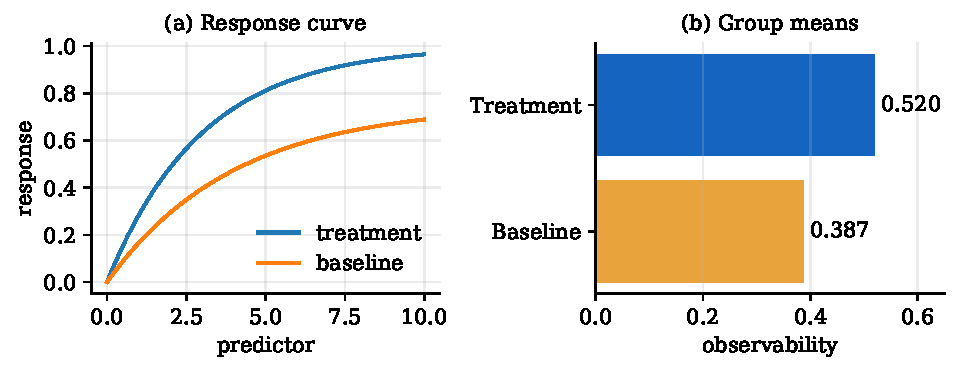
\includegraphics[width=\linewidth]{figures/example_figure.pdf}
  \caption{Example figure. Authored at \qty{6.5}{in} wide and included at
    \texttt{width=\textbackslash linewidth}, so its labels render at the same
    \qty{10}{pt} as the body text. Caption goes below the figure.}
  \label{fig:example}
\end{figure}

Figure~\ref{fig:example} shows the result. Tables are captioned ABOVE, and
TRB style is horizontal rules only -- no vertical rules.

\begin{table}[!ht]
  \centering
  \caption{Example table. Caption above; horizontal rules only.}
  \label{tab:example}
  \begin{tabular}{lrr}
    \toprule
    Condition & Mean & \(n\) \\
    \midrule
    Baseline    & 0.387 & 1\,204 \\
    Treatment   & 0.520 & 1\,198 \\
    Difference  & 0.133 & --     \\
    \bottomrule
  \end{tabular}
\end{table}

\section{Discussion}
Say what the numbers mean and, just as importantly, what they do not support.
Reviewers reward a paper that names its own limits before they have to.

\section{Conclusions}
Restate the finding and its scope. No new results here.

% ----------------------------------------------------------------------
% End matter. The AI-use disclosure is REQUIRED for the 2027 cycle --
% do not leave it out, and complete the matching field in the submission
% portal as well.
% ----------------------------------------------------------------------
\section*{Acknowledgments}
Funding sources and people who helped but are not authors.

\section*{Author Contributions}
Study conception and design: J.~Doe, R.~Roe; data collection: J.~Doe;
analysis and interpretation: J.~Doe, R.~Roe; draft preparation: J.~Doe.

\trbdataavailability{%
  State where the data are and how to get them. A published DOI that resolves
  today is worth more than a promise: deposit the data, publish it, and cite
  the DOI. A private reviewer link expires and leaves a dead credential in the
  version of record.}

\trbaidisclosure{%
  Disclose any generative AI tools used, what they were used for, and what they
  were not used for. Name the tools. State that the authors reviewed and
  verified all AI-assisted output and take full responsibility for the content.
  If no AI tools were used, say that instead -- the field is not optional.}

\bibliographystyle{trb}
\bibliography{references}

\end{document}
